%%This is a very basic article template.
%%There is just one section and two subsections.
\documentclass[a4paper,12pt,technote]{IEEEtran}
% weitere Pakete
% Grafiken aus PNG Dateien einbinden
\usepackage{graphicx}

% figure refs with section number
%\usepackage{chngcntr}
%\counterwithin{figure}{section}

% deutsche Silbentrennung
%\usepackage[ngerman]{babel}

% Eurozeichen einbinden
\usepackage[right]{eurosym}

% Umlaute unter UTF8 nutzen
\usepackage[utf8]{inputenc}

% Zeichenencoding
\usepackage[T1]{fontenc}

\usepackage{lmodern}
\usepackage{fix-cm}

% floatende Bilder ermöglichen
%\usepackage{floatflt}

%todos can be marked
\usepackage{todonotes}
% mehrseitige Tabellen ermöglichen
\usepackage{longtable}

% Unterstützung für Schriftarten
%\newcommand{\changefont}[3]{ 
%\fontfamily{#1} \fontseries{#2} \fontshape{#3} \selectfont}

% Packet für Seitenrandabständex und Einstellung für Seitenränder
%\usepackage{geometry}
%\geometry{left=3.5cm, right=2cm, top=2.5cm, bottom=2cm}

% Paket für Boxen im Text
\usepackage{fancybox}

\usepackage{lipsum}


% bricht lange URLs "schoen" um
\usepackage[hyphens,obeyspaces,spaces]{url}

% Paket für Textfarben
\usepackage{color}

% Mathematische Symbole importieren
\usepackage{amssymb}

% auf jeder Seite eine Überschrift (alt, zentriert)
%\pagestyle{headings}

% erzeugt Inhaltsverzeichnis mit Querverweisen zu den Kapiteln (PDF Version)
%\usepackage[bookmarksnumbered,pdftitle={\titleDocument},hyperfootnotes=false,hidelinks]{hyperref}
%\usepackage[bookmarksnumbered,pdftitle={\titleDocument},hyperfootnotes=false]{hyperref}
%\hypersetup{colorlinks, citecolor=red, linkcolor=blue, urlcolor=black}
%\hypersetup{colorlinks, citecolor=black, linkcolor= black, urlcolor=black}

% neue Kopfzeilen mit fancypaket
\usepackage{fancyhdr} %Paket laden
\pagestyle{fancy} %eigener Seitenstil
\fancyhf{} %alle Kopf- und Fußzeilenfelder bereinigen
\fancyhead[L]{\nouppercase{\leftmark}} %Kopfzeile links
\fancyhead[C]{} %zentrierte Kopfzeile
\fancyhead[R]{\thepage} %Kopfzeile rechts
\renewcommand{\headrulewidth}{0.4pt} %obere Trennlinie
%\fancyfoot[C]{\thepage} %Seitennummer
%\renewcommand{\footrulewidth}{0.4pt} %untere Trennlinie

% für Tabellen
\usepackage{array}

% Runde Klammern für Zitate
%\usepackage[numbers,round]{natbib}

% Schaltet den zusätzlichen Zwischenraum ab, den LaTeX normalerweise nach einem Satzzeichen einfügt.
%\frenchspacing

% Paket für Zeilenabstand
\usepackage{setspace}

% für Bildbezeichner
%\usepackage{capt-of}

% für Stichwortverzeichnis
\usepackage{makeidx}

% für Listings
\usepackage{listings}
%\lstset{
%  numbers=left,
%  numberstyle=\tiny,
%  numbersep=5pt,
%  breaklines=true,
%  breakatwhitespace,
%  keywordstyle=\color{black}\bfseries,
%  stringstyle=\sffamily,
%  showstringspaces=false,
%  basicstyle=\ttfamily\lst@ifdisplaystyle\footnotesize\else\normalsize\fi,
%  captionpos=b}
%\renewcommand{\lstlistingname}{Example}
%\AtBeginDocument{
%%\counterwithin{lstlisting}{section}
%}
%\setlength{\emergencystretch}{2pt}
% Indexerstellung
%\makeindex

% Abkürzungsverzeichnis
%\usepackage{nomencl}
%\let\abbrev\nomenclature

% Abkürzungsverzeichnis LiveTex Version
%\renewcommand{\nomname}{List of Abbreviations}
%\setlength{\nomlabelwidth}{.25\hsize}
%\renewcommand{\nomlabel}[1]{#1 \dotfill}
%\setlength{\nomitemsep}{-\parsep}
%\makenomenclature
%\makeglossary

% Abkürzungsverzeichnis TeTEX Version
% \usepackage[german]{nomencl}
% \makenomenclature
% %\makeglossary
% \renewcommand{\nomname}{Abkürzungsverzeichnis}
% \setlength{\nomlabelwidth}{.25\hsize}
% \renewcommand{\nomlabel}[1]{#1 \dotfill}
% \setlength{\nomitemsep}{-\parsep}

% Disable single lines at the start of a paragraph
%\clubpenalty = 10000
% Disable single lines at the end of a paragraph
%\widowpenalty = 10000
%\displaywidowpenalty = 10000

%\usepackage{titlesec}
%\subparagraph starting new line after heading
%\titleformat{\subparagraph}
%    {\normalfont\normalsize\bfseries}{\thesubparagraph}{1em}{}
%\titlespacing*{\subparagraph}{\parindent}{3.25ex plus 1ex minus .2ex}{.75ex plus .1ex}

% create additional subsection layer
%\makeatletter
%\renewcommand\paragraph{\@startsection{paragraph}{4}{\z@}
%	{-2.5ex\@plus -1ex \@minus -.25ex}
%	{1.25ex \@plus .25ex}
%	{\normalfont\normalsize\bfseries}}
%\makeatother
%\setcounter{secnumdepth}{4}
%\setcounter{tocdepth}{4}

\usepackage{etoolbox}
\lstset{showlines=true,
        basicstyle=\ttfamily}

\makeatletter
\AtBeginEnvironment{lstlisting}{%
\long\def\@makecaption#1#2{%
% test if is a for a figure or table
\ifx\@captype\@IEEEtablestring%
% if a table, do table caption
\footnotesize\bgroup\par\centering\@IEEEtabletopskipstrut{\normalfont\footnotesize #1}\\{\normalfont\footnotesize\scshape #2}\par\addvspace{0.5\baselineskip}\egroup%
\@IEEEtablecaptionsepspace
% if not a table, format it as a figure
\else
\@IEEEfigurecaptionsepspace
% 3/2001 use footnotesize, not small; use two nonbreaking spaces, not one
\setbox\@tempboxa\hbox{\normalfont\footnotesize {#1.}\nobreakspace\nobreakspace #2}%
\ifdim \wd\@tempboxa >\hsize%
% if caption is longer than a line, let it wrap around
\setbox\@tempboxa\hbox{\normalfont\footnotesize {#1.}\nobreakspace\nobreakspace}%
\parbox[b]{\hsize}{\normalfont\footnotesize\noindent\unhbox\@tempboxa#2}\medskip%
% if caption is shorter than a line, center if conference, left justify otherwise
\else%
\ifCLASSOPTIONconference \hbox to\hsize{\normalfont\footnotesize\hfil\box\@tempboxa\hfil}%
\else \hbox to\hsize{\normalfont\footnotesize\box\@tempboxa\hfil}\medskip%
\fi\fi\fi}}
\makeatother

\begin{document}
% hier werden die Trennvorschläge inkludiert
%\input{latex_einstellungen/trennung}

%syntax highlighting for additional languages
%\input{latex_einstellungen/systemverilog_code}
%\input{latex_einstellungen/e_code}

%Schriftart Helvetica
%\changefont{phv}{m}{n}

% Leere Seite am Anfang
%\newpage
%\thispagestyle{empty} % erzeugt Seite ohne Kopf- / Fusszeile
%\section*{ }

%use roman page numbers starting on this page
%\pagenumbering{roman}

% Titelseite %
%\include{latex_einstellungen/deckblatt}

% römische Numerierung
%\pagenumbering{arabic}

% 1.5 facher Zeilenabstand
%\onehalfspacing

% Sperrvermerk
%\input{sperrvermerk}
\title{Control and Status Register Files}
\author{Sebastian Wittka\\
Institute for Computer Engineering (ZITI) - Heidelberg University\\
Email: wittka@stud.uni-heidelberg.de}
\twocolumn[
\begin{@twocolumnfalse}
\maketitle
\end{@twocolumnfalse}]

% Einleitung / Abstract
\begin{abstract}
The steadily rising number of transistors on a chip increase the demand of generating functional units instead of designing everything manually. Therefore it is demonstated in this report how to fulfill this need for control and status register files. It is discussed why it is neccessary to generate such register files. The benefits and drawbacks of available generators are presented and especially the functionalities of the CAG Register File Generator are introduced.
\end{abstract}

% einfacher Zeilenabstand
%\singlespacing

% Eidesstattliche Erklärung
%\addcontentsline{toc}{section}{Declaration of Authorship}
%\include{erklaerung}

% Inhaltsverzeichnis anzeigen
%\newpage
%\tableofcontents
%\fancyhead[L]{}
% das Abbildungsverzeichnis
%\newpage
% Abbildungsverzeichnis soll im Inhaltsverzeichnis auftauchen
%\addcontentsline{toc}{section}{List of Figures}
% Abbildungsverzeichnis endgueltig anzeigen
%\listoffigures

% das Tabellenverzeichnis
%\newpage
% Abbildungsverzeichnis soll im Inhaltsverzeichnis auftauchen
%\addcontentsline{toc}{section}{Tabellenverzeichnis}
% \fancyhead[L]{Abbildungsverzeichnis / Abkürzungsverzeichnis} %Kopfzeile links
% Abbildungsverzeichnis endgueltig anzeigen
%\listoftables

%% WORKAROUND für Listings
%\makeatletter% --> De-TeX-FAQ
%\renewcommand*{\lstlistoflistings}{%
%  \begingroup
%    \if@twocolumn
%      \@restonecoltrue\onecolumn
%    \else
%      \@restonecolfalse
%    \fi
%    \lol@heading
%    \setlength{\parskip}{\z@}%
%    \setlength{\parindent}{\z@}%
%    \setlength{\parfillskip}{\z@ \@plus 1fil}%
%    \@starttoc{lol}%
%    \if@restonecol\twocolumn\fi
%  \endgroup
%}
%\makeatother% --> \makeatletter
% das Listingverzeichnis
%\newpage
% Listingverzeichnis soll im Inhaltsverzeichnis auftauchen
%\addcontentsline{toc}{section}{List of Examples}
%\fancyhead[L]{Abbildungs- / Tabellen- / Listingverzeichnis} %Kopfzeile links
%\renewcommand{\lstlistlistingname}{List of Examples}
%\lstlistoflistings
%%%%

% das Abkürzungsverzeichnis
%\newpage
% Abkürzungsverzeichnis soll im Inhaltsverzeichnis auftauchen
%\addcontentsline{toc}{section}{List of Abbreviations}
% das Abkürzungsverzeichnis entgültige Ausgeben
%\fancyhead[L]{Abkürzungsverzeichnis} %Kopfzeile links
%\input{latex_einstellungen/abkuezungen/abkuerzungen}
%\printnomenclature

% Definiert Stegbreite bei zweispaltigem Layout
%\setlength{\columnsep}{25pt}

%%%%%%% EINLEITUNG %%%%%%%%%%%%
%\twocolumn
%\newpage
%\fancyhead[L]{\nouppercase{\leftmark}} %Kopfzeile links

% 1,5 facher Zeilenabstand
%\onehalfspacing

%use arabic numbers starting with this page
%\pagenumbering{arabic}

% einzelne Kapitel
\section{Introduction}


\section{Control and Status Register Files}
\section{Register File Generation}\label{rf_generation}
RFs of state of the art hardware designs can easily contain several hundreds of CSRs. When an additional register is inserted during the design process, the entire address map of the RF has to be updated. Not only this has to be done in the hardware description, but also in all other parts involved in the design process like specification, documentation, and verification and simulation environment. This is both time-consuming and error prone. Therefore, it makes sense to have a single file containing the RF description with a high abstraction level. This file is then used to automatically generate all other required views.\\

Such RF descriptions can be drawn up using description languages like \emph{SystemRDL} or \emph{Spirit IP-XACT}, which are used in commercial RF generators. Where \emph{SystemRDL} is a language specific for RFs \cite{system_rdl} whereas \emph{Spirit IP-XACT} is not only able to describe RFs, but also the connections between hardware modules \cite{ip_xact}.\\

The main problem of these description languages is, that they do not support hierarchical RFs natively. When a single RF is placed centrally on a chip and the connected logic is spread across it, the routing delays between RF and logic become a huge concern. This can have a negative impact on the maximum frequency of the design. Hierarchical RFs can prevent this by placing the sub-RFs closer to the connected logic. Therefore the routing delays are reduced.\\
Additionally the syntax of both languages is not as clear as the one of the register file generator, which will be presented in the following section. Especially the one of \emph{Spirit IP-XACT} requires more characters to describe the same RF (fig.~\ref{fig::compare_syntax}).
\begin{figure}[h]
 \centering
 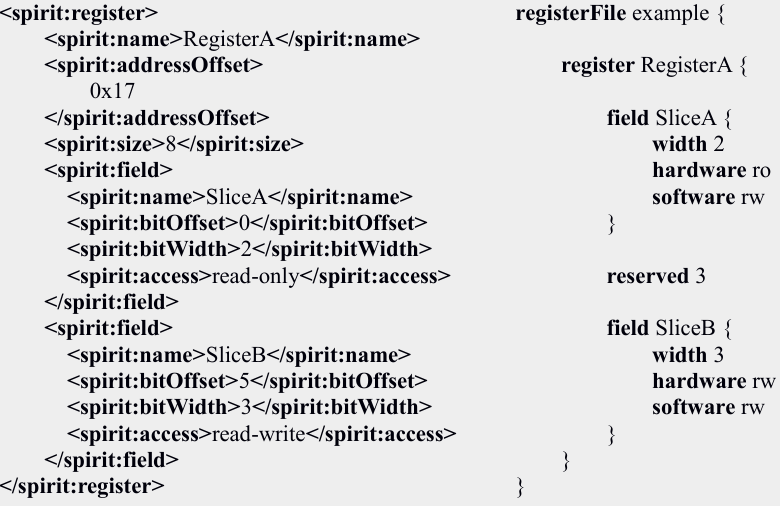
\includegraphics[width=252pt]{images/ip_vs_rfg.png}
 \caption{Spirit IP-XACT syntax compared to RFG \cite{markus_rfg}}
\label{fig::compare_syntax}
\end{figure}

\section{Register File Generator (RFG)}
\section{Conclusion}
It gets more and more important to generate uniform structures in the hardware design process to manage the increasing number of transistors available on a chip.\\
Thereby the RFG provides the functionality to generate the hardware description, verification model and documentation for RFs. This leads to a reduction in development time by avoiding time consuming and error prone tasks. The RF description syntax of the RFG is clearer than those of both SystemRDL and Spirit IP-XACT and supports hierarchical RFs, making it more suitable for large designs. Additionally, the verification model provides the ability to create reusable tests by accessing registers by their name instead of their address via the software interface. Furthermore, the RFG can easily be extended with generators for other parts of the RF.


\bibliographystyle{IEEEtran}
\bibliography{seminar}


%\include{2_uvm}

%\include{3_uvm_ml}

%\include{4_conclusion}


%\include{5_future_work}

%\include{beispiel}

%\onecolumn
% einfacher Zeilenabstand
%\singlespacing
% Literaturliste soll im Inhaltsverzeichnis auftauchen
%\addcontentsline{toc}{section}{References}
%\newpage

% Literaturverzeichnis anzeigen
%\renewcommand\refname{References}
%\bibliographystyle{plain}
%\bibliography{Seminar}
%% Index soll Stichwortverzeichnis heissen
% \newpage
% % Stichwortverzeichnis soll im Inhaltsverzeichnis auftauchen
% \addcontentsline{toc}{section}{Stichwortverzeichnis}
% \renewcommand{\indexname}{Stichwortverzeichnis}
% % Stichwortverzeichnis endgueltig anzeigen
% \printindex

%\onehalfspacing
% evtl. Anhang
%\newpage
%\addcontentsline{toc}{section}{Anhang}
%\fancyhead[L]{Anhang} %Kopfzeile links
%\input{anhang/anhang}

% leere Abschlussseite
%\newpage
%\thispagestyle{empty} % erzeugt Seite ohne Kopf- / Fusszeile
%\section*{ }


\end{document}
